%%%%%%%%%%%%%%%%%%%%%%%%%%%%%%%%%%%%%%%%%%%%%%%%%%%%%%%%%%%%%%%%%%%%%%%%%%%%%
%
%  System        : 
%  Module        : 
%  Object Name   : $RCSfile$
%  Revision      : $Revision$
%  Date          : $Date$
%  Author        : $Author$
%  Created By    : Robert Heller
%  Created       : Wed May 31 19:37:01 2017
%  Last Modified : <200210.1418>
%
%  Description 
%
%  Notes
%
%  History
% 
%%%%%%%%%%%%%%%%%%%%%%%%%%%%%%%%%%%%%%%%%%%%%%%%%%%%%%%%%%%%%%%%%%%%%%%%%%%%%
%
%    Copyright (C) 2017  Robert Heller D/B/A Deepwoods Software
%			51 Locke Hill Road
%			Wendell, MA 01379-9728
%
%    This program is free software; you can redistribute it and/or modify
%    it under the terms of the GNU General Public License as published by
%    the Free Software Foundation; either version 2 of the License, or
%    (at your option) any later version.
%
%    This program is distributed in the hope that it will be useful,
%    but WITHOUT ANY WARRANTY; without even the implied warranty of
%    MERCHANTABILITY or FITNESS FOR A PARTICULAR PURPOSE.  See the
%    GNU General Public License for more details.
%
%    You should have received a copy of the GNU General Public License
%    along with this program; if not, write to the Free Software
%    Foundation, Inc., 675 Mass Ave, Cambridge, MA 02139, USA.
%
% 
%
%%%%%%%%%%%%%%%%%%%%%%%%%%%%%%%%%%%%%%%%%%%%%%%%%%%%%%%%%%%%%%%%%%%%%%%%%%%%%

\documentclass[12pt,notitlepage,twoside]{book}
\usepackage{graphicx}
\usepackage{mathptm}
\usepackage{times}
\usepackage{makeidx}
\usepackage{ifpdf}
\ifpdf
\usepackage[pdftex,
            pagebackref=true,
            colorlinks=true,
            linkcolor=blue,
            unicode
           ]{hyperref}
\else
\usepackage[ps2pdf,
            pagebackref=true,
            colorlinks=true,
            linkcolor=blue,
            unicode
           ]{hyperref}
\usepackage{pspicture}
\fi
\usepackage{url}
\pagestyle{headings}
\makeindex
\emergencystretch=50pt
\setcounter{tocdepth}{3}
\setcounter{secnumdepth}{3}
\includeonly{SMCSenseHAT,QuadSSSQuadIn,MCP23017,OctalLEDDriver,QuadSMCSenseHat,LCCCANCape,QuadSMCSenseCape,QuadSMCSenseHat,PocketBeagleQuadSMCSense,ESP32QuadSMCSense,ESP32-PWMHalfSiding}
\begin{document}
\title{Railroad Circuits for the Raspberry Pi, Beagle Bone Black, Pocket Beagle, and ESP32}
\author{Robert Heller \\ The Country Robot \\ Wendell, MA, USA}
\date{\today}
\begin{titlepage}

\maketitle

\clearpage

This documentation was prepared with \LaTeX.

\vspace{.25in}


{\small Copyright \copyright 2017-2019 by Robert Heller D/B/A The Country Robot}
\vspace{.25in}

All rights reserved.  Permission is granted to copy this document in
electronic form only, so long as it is with the software it
documents. 

\vspace{.125in}

The author, Robert Heller, may be contacted electronically (E-Mail) via
\url{mailto:heller@thecountryrobot.com}.

\vspace{.25in}

The Country Robot's web site URL: \url{http://www.thecountryrobot.com/}.

\thispagestyle{empty}
\setcounter{page}{0}
\clearpage

\end{titlepage}

\pagenumbering{roman}
\tableofcontents
\listoffigures
\listoftables
\cleardoublepage
\chapter*{Preface}
\addcontentsline{toc}{chapter}{Preface}

This booklet describes a collection of circuit boards I designed to make use 
of Raspberry Pi GPIO pins to be used in the control of a model railroad 
layout.  I am not formally trained as an electronics engineer, but these 
circuits are fairly simple and are readily cribbed from the data sheets of the 
various microchips used.  If someone who is a trained electronics engineer 
finds something wrong, I would of course like to hear about it.

\cleardoublepage
\pagenumbering{arabic}
\chapter{General Information}

Many of these boards are add on boards for a Raspberry Pi ``B'' model, 
one with a 40-pin header and have the mechanical form factor of a Raspberry Pi 
``HAT''.  Since none of them have an eeprom on them, they are technically not 
actual ``HATs''.  These boards can be ``stacked'', with some limitations, as 
indicated in their respective chapters, mainly because some of these boards 
are hard wired to use specific GPIO pins.  It is therefore possible to use 
``stacking'' (or ``stack through'') headers, headers that are both female 
sockets and male pins.  The end user has a choice of headers to use: standard 
female only headers, long female only headers, standard ``stacking'' headers 
or long/tall ``stacking'' headers.  In the chapters for each board in the 
parts list section, I list the various header options, with part numbers and 
suppliers.  Other boards are stackable ``Capes'' for the Beagle Bone Black. 
Again, since many of these boards are stackable, ``stacking'' (or ``stack 
through'') headers can be used.  Still other boards are for the Pocket Beagle 
and the ESP32 devkit board.  These latter are not meant to be stackable and 
for these, the add on board goes \textit{under} the processor board.  Unlike 
the Raspberry Pi and Beagle Bone Black, these smaller boards have no mounting 
holes, but the ``add on'' boards do.  Also for these smaller boards the add 
on boards provide power to the processor board.

Another place where the end user has choices is in the terminal blocks.  With 
some exceptions (mostly for higher power cases), all of the terminal blocks 
are specified as .1'' (2.54mm) pitch screw terminals.  It is possible to 
substitute other .1'' (2.54mm) pitch connections, including vertical or right 
angle pin arrays or even spring terminals.  This will depend on what sort of 
interconnection technology the end user would prefer.  In the parts list will 
be the various alternative options.

All of the boards use mostly through-hole parts and should be fairly easy to
hand solder with a basic good quality soldering iron. All of the components
are standard and readily available from various suppliers (like Mouser or
Digi-Key).

Most of the boards have mounting holes.  The mounting holes on the HAT-like 
boards align over the mounting holes in the Raspberry Pi.  Using standard 
height headers allows about 3/8'' between boards and using tall headers allows 
1/2'' between boards.  It is probably a good idea to use spacer hardware to 
secure the boards.  Male/female 4-40 threaded hex spacers work quite well, 
although the boards are designed to use M2.5 hardware (Adafruit sells M2.5 
male/female threaded hex spacers in pairs).

%%%%%%%%%%%%%%%%%%%%%%%%%%%%%%%%%%%%%%%%%%%%%%%%%%%%%%%%%%%%%%%%%%%%%%%%%%%%%
%
%  System        : 
%  Module        : 
%  Object Name   : $RCSfile$
%  Revision      : $Revision$
%  Date          : $Date$
%  Author        : $Author$
%  Created By    : Robert Heller
%  Created       : Wed May 31 20:05:00 2017
%  Last Modified : <170531.2304>
%
%  Description 
%
%  Notes
%
%  History
% 
%%%%%%%%%%%%%%%%%%%%%%%%%%%%%%%%%%%%%%%%%%%%%%%%%%%%%%%%%%%%%%%%%%%%%%%%%%%%%
%
%    Copyright (C) 2017  Robert Heller D/B/A Deepwoods Software
%			51 Locke Hill Road
%			Wendell, MA 01379-9728
%
%    This program is free software; you can redistribute it and/or modify
%    it under the terms of the GNU General Public License as published by
%    the Free Software Foundation; either version 2 of the License, or
%    (at your option) any later version.
%
%    This program is distributed in the hope that it will be useful,
%    but WITHOUT ANY WARRANTY; without even the implied warranty of
%    MERCHANTABILITY or FITNESS FOR A PARTICULAR PURPOSE.  See the
%    GNU General Public License for more details.
%
%    You should have received a copy of the GNU General Public License
%    along with this program; if not, write to the Free Software
%    Foundation, Inc., 675 Mass Ave, Cambridge, MA 02139, USA.
%
% 
%
%%%%%%%%%%%%%%%%%%%%%%%%%%%%%%%%%%%%%%%%%%%%%%%%%%%%%%%%%%%%%%%%%%%%%%%%%%%%%

\chapter{SMCSenseHAT: Stall Motor Control and Sense HAT}

This is a circuit board to for an add-on board for a Raspberry Pi B+ that will
control  two  stall-motor  turnout  motors for a model  railroad.  It also has
sense  logic to return the state of the  turnouts,  using one pole of the DPDT
contacts in the stall-motor (typical of Tortoise stall-motors).

The circuit board uses a 40pin header socket to connect to the 40pin header on
the  Raspberry Pi B+ and can use a  stack-through  header to allow  additional
boards to be stacked on top of it.

\section{GPIO Pins Used and stacking restrictions.}

This board uses four GPIO pins:

\begin{description}
\item[WiringPi 0, BCM 17] Motor Select 1: select the position of stall motor 
1. 
\item[WiringPi 1, BCM 18] Motor Select 2: select the position of stall motor 
2. 
\item[WiringPi 2, BCM 27] Point Sense 1: return the state of the points for 
stall motor 1. 
\item[WiringPi 3, BCM 22] Point Sense 2: return the state of the points for 
stall motor 2. 
\end{description}

Each of the motor drive circuits is through a transistor that can handle 1 amp 
continuious colector current, which is way more needed to drive typical stall 
motor.  It is enough to drive a pair of stall motors, wired in parallel as 
would be the case for a cross over.

Because this board is hardwired to use four specicic GPIO pins it is not 
possible to use two or more of these boards on given Raspberry Pi.  But in the 
SMCSenseHAT1 directory is a nearly identical board, that uses a different set 
of four GPIO pins:

\begin{description}
\item[WiringPi 4, BCM 23] Motor Select 1: select the position of stall motor 
1. 
\item[WiringPi 5, BCM 24] Motor Select 2: select the position of stall motor 
2. 
\item[WiringPi 6, BCM 25] Point Sense 1: return the state of the points for 
stall motor 1. 
\item[WiringPi 7, BCM 4] Point Sense 2: return the state of the points for 
stall motor 2. 
\end{description}

It is possible use one each of the SMCSenseHAT and SMCSenseHAT1 boards to 
handle four separate turnouts.  You should only connect at most one of each of 
these boards on a single Raspberry Pi.



%%%%%%%%%%%%%%%%%%%%%%%%%%%%%%%%%%%%%%%%%%%%%%%%%%%%%%%%%%%%%%%%%%%%%%%%%%%%%
%
%  System        : 
%  Module        : 
%  Object Name   : $RCSfile$
%  Revision      : $Revision$
%  Date          : $Date$
%  Author        : $Author$
%  Created By    : Robert Heller
%  Created       : Wed May 31 20:07:09 2017
%  Last Modified : <171103.1610>
%
%  Description 
%
%  Notes
%
%  History
% 
%%%%%%%%%%%%%%%%%%%%%%%%%%%%%%%%%%%%%%%%%%%%%%%%%%%%%%%%%%%%%%%%%%%%%%%%%%%%%
%
%    Copyright (C) 2017  Robert Heller D/B/A Deepwoods Software
%			51 Locke Hill Road
%			Wendell, MA 01379-9728
%
%    This program is free software; you can redistribute it and/or modify
%    it under the terms of the GNU General Public License as published by
%    the Free Software Foundation; either version 2 of the License, or
%    (at your option) any later version.
%
%    This program is distributed in the hope that it will be useful,
%    but WITHOUT ANY WARRANTY; without even the implied warranty of
%    MERCHANTABILITY or FITNESS FOR A PARTICULAR PURPOSE.  See the
%    GNU General Public License for more details.
%
%    You should have received a copy of the GNU General Public License
%    along with this program; if not, write to the Free Software
%    Foundation, Inc., 675 Mass Ave, Cambridge, MA 02139, USA.
%
% 
%
%%%%%%%%%%%%%%%%%%%%%%%%%%%%%%%%%%%%%%%%%%%%%%%%%%%%%%%%%%%%%%%%%%%%%%%%%%%%%

\chapter{QuadSSSQuadIn: Quad SSR and Quad 5V Input HAT}

This is a circuit board to for an add-on board for a Raspberry Pi B+ that will
add four 5V logic inputs and four Solid State Relays, using a MCP23008 I2C I/O 
expander.  There is a jumper header to set one of eight addresses for the 
MCP23008 chip.  This allows using more than one of this board or any other 
board featuring a MCP23008 or MCP23016 or MCP23017 chip (up to eight total).

The circuit board uses a 40pin header socket to connect to the 40pin header on
the  Raspberry Pi B+ and can use a  stack-through  header to allow  additional
boards to be stacked on top of it.

\section{Circuit Description}                                                  
 
\begin{figure}[hbpt]\begin{centering}%
\includegraphics[width=5in]{QuadSSSQuadIn.pdf}
\caption{Circuit Diagram of the QuadSSSQuadIn}
\end{centering}\end{figure}
This circuit uses a MCP23008 to expand the Raspberry Pis I/O to 8 additional 
I/O pins.  Four of these pins (0-3) are used to drive a pair of dual 
opto-isolated SSR chip and the remaining 4 (4-7) are driven by a input buffer 
chip that can be driven with 5V logic.  The SSRs can be used to switch 
arbituary trackside devices, since the output side of the SSRs are rated upto 
+/- 400 volts at up to 0.1 Amp (100ma).  The 5V logic inputs are compatible 
with many sensor boards available (partitularly occupancy detector circuits).

\section{Parts List}

\begin{table}[htdp]
\begin{centering}\begin{tabular}{|l|l|p{1in}|l|p{.5in}|}
\hline
Value&Qty&Refs&Mouser Part Number&Adafruit Part Number\\
\hline
.1 uf&3&C1 C2 C3&21RZ310-RC&\\
\hline
ASSR-4128&2&IC1 IC2&630-ASSR-4128-002E&\\
\hline
RPi GPIO&1&J0&855-M20-6102045&2223\\
\hline
CONN 3X2&1&J1&517-929836-02-03&\\
\hline
330 Ohms&1&RP1&652-4608X-AP2-331LF&\\
\hline
10K Ohms&2&RR1 RR2&652-4605X-1LF-10K&\\
\hline
CONN 8&1&T1&651-1725711&\\
\hline
CONN 6&1&T2&651-1725698&\\
\hline
MCP23008&1&U1&579-MCP23008-E/P&\\
\hline
74LV125AN&1&U2&595-SN74LV125AN&\\
\hline
\end{tabular}
\caption{Parts list for QuadSSSQuadIn boards.}
\end{centering}\end{table}\footnote{Mouser Project link: 
\url{http://www.mouser.com/ProjectManager/ProjectDetail.aspx?AccessID=97fe7b85dc}.}

The only parts that might be substituted are J0 (the RPi GPIO Header), and T1
and T2 (the I/O terminals). The parts listed are for the stacking headers for 
the RPi GPIO Header, and screw terminals for the I/O terminals.  Feel free to 
select a non-stacking header for the RPi GPIO Header and to select either pin 
arrays or spring terminals for the T1 and T2.                   

\section{Circuit Board Layout}

\begin{figure}[hbpt]\begin{centering}%
\includegraphics[width=5in]{QuadSSSQuadIn3DTop.png}
\caption{3D rendering of the QuadSSSQuadIn board}
\end{centering}\end{figure}
\begin{figure}[hbpt]\begin{centering}%
\includegraphics[width=5in]{QuadSSSQuadIn.png}
\caption{Fabrication image of the QuadSSSQuadIn board}
\end{centering}\end{figure}
Board assembly is straight forward.  You need to be careful orienting the ICs, 
noting that the SSRs are opositely oriented from the other ICs.  Also the 
SIP resistor arrays need to be carefully oriented -- the dot marks pin 1, 
which is indicated on the board with a square pad\footnote{The first batch of 
the boards I ordered used the wrong PCB modules for the terminals and the 
holes are too small for the screw terminal pins to go all the way in.  They 
can be ``jammed'' in enough to be soldered. Pin arrays fit a little better, 
but still need some effort to seat.  The next batch I order will not have this 
problem.}. 


%%%%%%%%%%%%%%%%%%%%%%%%%%%%%%%%%%%%%%%%%%%%%%%%%%%%%%%%%%%%%%%%%%%%%%%%%%%%%
%
%  System        : 
%  Module        : 
%  Object Name   : $RCSfile$
%  Revision      : $Revision$
%  Date          : $Date$
%  Author        : $Author$
%  Created By    : Robert Heller
%  Created       : Wed May 31 20:09:46 2017
%  Last Modified : <171104.0938>
%
%  Description 
%
%  Notes
%
%  History
% 
%%%%%%%%%%%%%%%%%%%%%%%%%%%%%%%%%%%%%%%%%%%%%%%%%%%%%%%%%%%%%%%%%%%%%%%%%%%%%
%
%    Copyright (C) 2017  Robert Heller D/B/A Deepwoods Software
%			51 Locke Hill Road
%			Wendell, MA 01379-9728
%
%    This program is free software; you can redistribute it and/or modify
%    it under the terms of the GNU General Public License as published by
%    the Free Software Foundation; either version 2 of the License, or
%    (at your option) any later version.
%
%    This program is distributed in the hope that it will be useful,
%    but WITHOUT ANY WARRANTY; without even the implied warranty of
%    MERCHANTABILITY or FITNESS FOR A PARTICULAR PURPOSE.  See the
%    GNU General Public License for more details.
%
%    You should have received a copy of the GNU General Public License
%    along with this program; if not, write to the Free Software
%    Foundation, Inc., 675 Mass Ave, Cambridge, MA 02139, USA.
%
% 
%
%%%%%%%%%%%%%%%%%%%%%%%%%%%%%%%%%%%%%%%%%%%%%%%%%%%%%%%%%%%%%%%%%%%%%%%%%%%%%

\chapter{MCP23017Hat: 16 bit GPIO expander HAT}

This is a circuit board to for an add-on board for a Raspberry Pi B+ that will 
add 16 3V GPIO pins, using a MCP23017 I2C I/O expander. There is a jumper 
header to set one of eight addresses for the MCP23017 chip.  This allows using 
more than one of this board or any other board featuring a MCP23008 or 
MCP23016 or MCP23017 chip (up to eight total). 

The circuit board uses a 40pin header socket to connect to the 40pin header on 
the  Raspberry Pi B+ and can use a  stack-through  header to allow  additional 
boards to be stacked on top of it.                                             
 
\section{Circuit Description}          

\begin{figure}[hbpt]\begin{centering}%
\includegraphics[width=5in]{MCP23017.pdf}
\caption{Circuit Diagram of the MCP23017}
\end{centering}\end{figure}
This circuit uses a MCP23017 to expand the Raspberry Pis I/O to 16 additional 
I/O pins. The 16 3V logic pins are simply brought out to screw terminals, 
along with the 3V and ground connections (useful for logic reference).

\section{Parts List}

\begin{table}[htdp]
\begin{centering}\begin{tabular}{|l|l|p{1in}|l|p{.5in}|}
\hline
Value&Qty&Refs&Mouser Part Number&Adafruit Part Number\\
\hline
.1 uf&1&C1&21RZ310-RC&\\
\hline
RPi GPIO&1&J0&855-M20-6102045&2223\\
\hline
Address Jumper&1&J1&517-929836-02-03&\\
\hline
10K Ohms&1&RR1&652-4605X-1LF-10K&\\
\hline
GP0;GP1&2&T1 T2&651-1725737 or 2x 651-1725685&\\
\hline
MCP23017&1&U1&579-MCP23017-E/SP&\\
\hline
\end{tabular}
\caption{Parts list for MCP23017 boards.}
\end{centering}\end{table}\footnote{Mouser Project link: 
\url{http://www.mouser.com/ProjectManager/ProjectDetail.aspx?AccessID=25df06786a}.}

The only parts that might be substituted are J0 (the RPi GPIO Header), and T1
and T2 (the I/O terminals). The parts listed are for the stacking headers for 
the RPi GPIO Header, and screw terminals for the I/O terminals.  Feel free to 
select a non-stacking header for the RPi GPIO Header and to select either pin 
arrays or spring terminals for the T1 and T2.                   

\section{Circuit Board Layout}

\begin{figure}[hbpt]\begin{centering}%
\includegraphics[width=5in]{MCP230173DTop.png}
\caption{3D rendering of the MCP23017 board}
\end{centering}\end{figure}
\begin{figure}[hbpt]\begin{centering}%
\includegraphics[width=5in]{MCP23017.png}
\caption{Fabrication image of the MCP23017 board}
\end{centering}\end{figure}
Board assembly is straight forward. You need to be careful orienting the IC.
Also the SIP resistor array needs to be carefully oriented -- the dot marks
pin 1, which is indicated on the board with a square pad. 

\section{Downloadables and Software Support}

Full design information is available on GitHub here:
\url{https://github.com/RobertPHeller/RPi-RRCircuits/tree/master/MCP23017Hat}.

This board is supported by the Model Railroad System\footnote{Available as a 
free download from Deepwoods Software at this web address: 
\url{http://www.deepsoft.com/home/products/modelrailroadsystem/}.}
\texttt{OpenLCB\_PiMCP23017} and \texttt{OpenLCB\_PiMCP23017\_signal} daemons.
A basic XML file for it is included in its GitHub folder. 



%%%%%%%%%%%%%%%%%%%%%%%%%%%%%%%%%%%%%%%%%%%%%%%%%%%%%%%%%%%%%%%%%%%%%%%%%%%%%
%
%  System        : 
%  Module        : 
%  Object Name   : $RCSfile$
%  Revision      : $Revision$
%  Date          : $Date$
%  Author        : $Author$
%  Created By    : Robert Heller
%  Created       : Fri Nov 3 11:46:41 2017
%  Last Modified : <171104.0951>
%
%  Description 
%
%  Notes
%
%  History
% 
%%%%%%%%%%%%%%%%%%%%%%%%%%%%%%%%%%%%%%%%%%%%%%%%%%%%%%%%%%%%%%%%%%%%%%%%%%%%%
%
%    Copyright (C) 2017  Robert Heller D/B/A Deepwoods Software
%			51 Locke Hill Road
%			Wendell, MA 01379-9728
%
%    This program is free software; you can redistribute it and/or modify
%    it under the terms of the GNU General Public License as published by
%    the Free Software Foundation; either version 2 of the License, or
%    (at your option) any later version.
%
%    This program is distributed in the hope that it will be useful,
%    but WITHOUT ANY WARRANTY; without even the implied warranty of
%    MERCHANTABILITY or FITNESS FOR A PARTICULAR PURPOSE.  See the
%    GNU General Public License for more details.
%
%    You should have received a copy of the GNU General Public License
%    along with this program; if not, write to the Free Software
%    Foundation, Inc., 675 Mass Ave, Cambridge, MA 02139, USA.
%
% 
%
%%%%%%%%%%%%%%%%%%%%%%%%%%%%%%%%%%%%%%%%%%%%%%%%%%%%%%%%%%%%%%%%%%%%%%%%%%%%%

\chapter{OctalLEDDriver: Octal LED (Common Cathode) driver board.}

This is a standalone board that takes eight 3V GPIO pins (such as from a MCP23017 
or MCP23008 HAT board or just from eight of a Raspberry Pi's GPIO pins and buffers 
them to drive up to eight LEDs from a 5V supply.  It is specificly designed for 
common cathode signals.  It has a ten position screw terminal at one end, for 
GND, GPIO 0 through 7, and +3V (it does not actually use the +3V connection, 
but includes it to match the terminals on a MCP23017 or MCP23008 HAT board and 
thus can support the use of ten conductor cable or pin header connectors, 
etc.).  At the other end it is two sets of +5V and ground terminals (to allow 
for daisy chaining the +5V supply bus), and nine position screw terminal for 
LEDs 0 though 7 and the common cathode (K), which is ground.

\section{Circuit Description}

\begin{figure}[hbpt]\begin{centering}%
\includegraphics[width=5in]{OctalLEDDriver.pdf}
\caption{Circuit Diagram of the OctalLEDDriver}
\end{centering}\end{figure}
The circuit is just eight driver circuits, each featuring a NPN and a PNP
transistor, that level shift and buffer the 3V logic to 20 milliamp, 5V LED
drive circuits. The circuits include a current limiting series resistor, so
there is no need to include external resistors on your LEDs. The circuit
assumes 2V LEDs (typical of standard red, green, and yellow LEDs).

\section{Parts List}

\begin{table}[htdp]
\begin{centering}\begin{tabular}{|l|l|p{1in}|l|}
\hline
Value&Quantity&References&Mouser Part Number\\
\hline
MPQ6002&4&Q1 Q2 Q3 Q4&610-MPQ6002\\
\hline
15K Ohms&8&R1 R5 R9 R13 R17 R21 R25 R29&603-CFR-25JR-5215K\\
\hline
10K Ohms&8&R2 R6 R10 R14 R18 R22 R26 R30&603-CFR-25JR-5210K\\
\hline
2K Ohms&8&R3 R7 R11 R15 R19 R23 R27 R31&603-CFR-25JR-522K\\
\hline
150 Ohms&8&R4 R8 R12 R16 R20 R24 R28 R32&588-OK1515E-R52\\
\hline
GPIO (3.3V)&1&T1&651-1725737 or 2x 651-1725685 \\
\hline
LED Power (5V)&2&T2 T4&651-1725656\\
\hline
LEDs (Common Cathode)&1&T3&651-1725724\\
\hline
\end{tabular}
\caption{Parts list for OctalLEDDriver boards.}
\end{centering}\end{table}\footnote{Mouser Project link: 
\url{http://www.mouser.com/ProjectManager/ProjectDetail.aspx?AccessID=f337ca3247}.}

The only parts that might be substituted are the screw terminal boards. Feel 
free to select either pin arrays or spring terminals for the terminals.

\section{Circuit Board Layout}

\begin{figure}[hbpt]\begin{centering}%
\includegraphics[width=5in]{OctalLEDDriver3DTop.png}
\caption{3D rendering of the OctalLEDDriver board}
\end{centering}\end{figure}
\begin{figure}[hbpt]\begin{centering}%
\includegraphics[width=5in]{OctalLEDDriver.png}
\caption{Fabrication image of the OctalLEDDriver board}
\end{centering}\end{figure}
Board assembly is straight forward. You need to be careful orienting the quad 
transistors. 

\section{Downloadables}

Full design information is available on GitHub here:
\url{https://github.com/RobertPHeller/RPi-RRCircuits/tree/master/OctalLEDDriver}.




%%%%%%%%%%%%%%%%%%%%%%%%%%%%%%%%%%%%%%%%%%%%%%%%%%%%%%%%%%%%%%%%%%%%%%%%%%%%%
%
%  System        : 
%  Module        : 
%  Object Name   : $RCSfile$
%  Revision      : $Revision$
%  Date          : $Date$
%  Author        : $Author$
%  Created By    : Robert Heller
%  Created       : Mon Jul 15 17:34:14 2019
%  Last Modified : <190803.1514>
%
%  Description 
%
%  Notes
%
%  History
% 
%%%%%%%%%%%%%%%%%%%%%%%%%%%%%%%%%%%%%%%%%%%%%%%%%%%%%%%%%%%%%%%%%%%%%%%%%%%%%
%
%    Copyright (C) 2019  Robert Heller D/B/A Deepwoods Software
%			51 Locke Hill Road
%			Wendell, MA 01379-9728
%
%    This program is free software; you can redistribute it and/or modify
%    it under the terms of the GNU General Public License as published by
%    the Free Software Foundation; either version 2 of the License, or
%    (at your option) any later version.
%
%    This program is distributed in the hope that it will be useful,
%    but WITHOUT ANY WARRANTY; without even the implied warranty of
%    MERCHANTABILITY or FITNESS FOR A PARTICULAR PURPOSE.  See the
%    GNU General Public License for more details.
%
%    You should have received a copy of the GNU General Public License
%    along with this program; if not, write to the Free Software
%    Foundation, Inc., 675 Mass Ave, Cambridge, MA 02139, USA.
%
% 
%
%%%%%%%%%%%%%%%%%%%%%%%%%%%%%%%%%%%%%%%%%%%%%%%%%%%%%%%%%%%%%%%%%%%%%%%%%%%%%

\chapter{LCCCANCape: LCC CAN Tranceiver Cape}

\section{GPIO Pins Used and stacking restrictions.}

This board uses two pins on header P9: 24 and 26 in pin mux mode2, which makes 
pin 24 Can1 RX, and pin 26 Can1 TX.  Only one of these capes can be on any 
Beagle Bone Black.


\section{Circuit Description}

\begin{figure}[hbpt]\begin{centering}%                                         
\includegraphics[width=5in]{LCCCANCape-1.pdf}                               
\caption{Circuit Diagram of the LCCCANCape}                               
\end{centering}\end{figure}                                                    
This circuit contains two sectins.  There is the transciever section, which 
includes the transciver itself, the termination block, the two RJ45 jacks, and 
two terminal blocks for injecting and tapping into the power carried in the 
CAT 5 cable.  Power is not used to power the Beagle Bone Black.  The other 
section is the Cape EErom circuit.  The Cape EEProm contains         
information about the cape and the name and version of the overlay that needs  
to be loaded by uBoot.  

\clearpage

\section{Parts List}

\begin{table}[htdp]
\begin{centering}\begin{tabular}{|l|l|p{1in}|l|}
\hline
Value&Quantity&References&Mouser Part Number \\
\hline
.1 uf&1&C8&581-SR201C104KARTR1 \\
\hline
WP 1 0&1&P2&649-67996-406HLF \\
\hline
5.6K Ohms&2&R3 R4&603-CFR-25JR-525K6 \\
\hline
4.75K Ohms&3&R5 R6 R7&603-CFR-25JR-524K7 \\
\hline
10K Ohms&1&R8&603-CFR-25JR-5210K \\
\hline
CAT24C256W&1&U9&698-CAT24C256WI-GT3 \\
\hline
.1 uf&1&C1&21RZ310-RC \\
\hline
15 uf 63V&1&C2&710-860080773002 \\
\hline
47 nf&1&C3&75-1C10Z5U473M050B \\
\hline
SB240E&2&D1 D2&625-SB240-E3 \\
\hline
RJ45&2&J1 J2&710-615008144221 \\
\hline
Termination&1&JP1&649-67997-404HLF \\
\hline
60 Ohms&2&R1 R2&71-RN60C60R0B/R \\
\hline
+ 15 in -;+ 15 out -&2&T1 T2&651-1725656 \\
\hline
TCAN332DR&1&U1&595-TCAN332DR \\
\hline
SN65HVD233-HT&1&U2&595-SN65HVD233SJD \\
\hline
BeagleBone\_Black\_Header&2&''P8 P9''&200-ESQ12314GD \\
\hline
\end{tabular}
\caption{Parts list for LCCCANCape board.}
\end{centering}\end{table}\footnote{Mouser Project links: 
\url{http://www.mouser.com/ProjectManager/ProjectDetail.aspx?AccessID=ae58a2d985},
\url{http://www.mouser.com/ProjectManager/ProjectDetail.aspx?AccessID=522a1259b2}.}


The only parts that might be substituted are P8 and P9 (the Beagle Bone Black
Headers). The parts listed are for the stacking headers for the Beagle Bone
Black Headers. Feel free to select a non-stacking header for the Beagle Bone
Black Headers.


\section{Circuit Board Layout}

\begin{figure}[hbpt]\begin{centering}%
\includegraphics[width=5in]{LCCCANCape3DTop.png}
\caption{3D rendering of the LCCCANCape board}
\end{centering}\end{figure}
\begin{figure}[hbpt]\begin{centering}%
\includegraphics[width=5in]{LCCCANCape.png}
\caption{Fabrication image of the LCCCANCape board}
\end{centering}\end{figure}
Board assembly is straight forward. You need to be careful orienting the ICs
and the electrolytic capacitor.


\section{Downloadables and Software Support}

Full design information is available on GitHub here:
\url{https://github.com/RobertPHeller/RPi-RRCircuits/tree/master/LCCCANCape}.

This board is supported by both the Model Railroad System 
(\url{https://github.com/RobertPHeller/ModelRRSystem}) and the OpenMRN 
(\url{https://github.com/bakerstu/openmrn}).

%%%%%%%%%%%%%%%%%%%%%%%%%%%%%%%%%%%%%%%%%%%%%%%%%%%%%%%%%%%%%%%%%%%%%%%%%%%%%
%
%  System        : 
%  Module        : 
%  Object Name   : $RCSfile$
%  Revision      : $Revision$
%  Date          : $Date$
%  Author        : $Author$
%  Created By    : Robert Heller
%  Created       : Mon Jul 15 17:33:37 2019
%  Last Modified : <190716.1304>
%
%  Description 
%
%  Notes
%
%  History
% 
%%%%%%%%%%%%%%%%%%%%%%%%%%%%%%%%%%%%%%%%%%%%%%%%%%%%%%%%%%%%%%%%%%%%%%%%%%%%%
%
%    Copyright (C) 2019  Robert Heller D/B/A Deepwoods Software
%			51 Locke Hill Road
%			Wendell, MA 01379-9728
%
%    This program is free software; you can redistribute it and/or modify
%    it under the terms of the GNU General Public License as published by
%    the Free Software Foundation; either version 2 of the License, or
%    (at your option) any later version.
%
%    This program is distributed in the hope that it will be useful,
%    but WITHOUT ANY WARRANTY; without even the implied warranty of
%    MERCHANTABILITY or FITNESS FOR A PARTICULAR PURPOSE.  See the
%    GNU General Public License for more details.
%
%    You should have received a copy of the GNU General Public License
%    along with this program; if not, write to the Free Software
%    Foundation, Inc., 675 Mass Ave, Cambridge, MA 02139, USA.
%
% 
%
%%%%%%%%%%%%%%%%%%%%%%%%%%%%%%%%%%%%%%%%%%%%%%%%%%%%%%%%%%%%%%%%%%%%%%%%%%%%%

\chapter{QuadSMCSenseHat: Quad Motor Control and Sense HAT}

This is a circuit board to for an add-on board for a Raspberry Pi B+ that will
control four stall-motor turnout motors for a model railroad. It also has
sense logic to return the state of the turnouts, using one pole of the DPDT
contacts in the stall-motor (typical of Tortoise stall-motors).

The circuit board uses a 40pin header socket to connect to the 40pin header on
the  Raspberry Pi B+ and can use a  stack-through  header to allow  additional
boards to be stacked on top of it.

\section{GPIO Pins Used and stacking restrictions.}

This board uses eight GPIO pins:

\begin{description}
\item[WiringPi 0, BCM 17] Motor Select 1: select the position of stall motor 
1. 
\item[WiringPi 1, BCM 18] Motor Select 2: select the position of stall motor 
2. 
\item[WiringPi 2, BCM 27] Point Sense 1: return the state of the points for 
stall motor 1. 
\item[WiringPi 3, BCM 22] Point Sense 2: return the state of the points for 
stall motor 2. 
\item[WiringPi 4, BCM 23] Motor Select 3: select the position of stall motor 
3. 
\item[WiringPi 5, BCM 24] Motor Select 4: select the position of stall motor 
4. 
\item[WiringPi 6, BCM 25] Point Sense 3: return the state of the points for 
stall motor 3. 
\item[WiringPi 7, BCM 4] Point Sense 4: return the state of the points for 
stall motor 4. 
\end{description}

Each of the motor drive circuits is through a TC4428, which can drive up to
1.5A, which is way more needed to drive typical stall motor. It is enough to
drive a pair of stall motors, wired in parallel as would be the case for a
cross over. 

Because this board is hardwired to use eight specific GPIO pins it is not 
possible to use two or more of these boards on given Raspberry Pi.

\section{Circuit Description}

\begin{figure}[hbpt]\begin{centering}%
\includegraphics[width=5in]{QuadSMCSenseHat.pdf}
\caption{Circuit Diagram of the QuadSMCSenseHat}
\end{centering}\end{figure}
This circuit contains two sections.  There is an output section that contains 
four TC4428 chips.  Each chip has a non-inverting and an inverting driver. The 
inputs of both drivers are connected to one of the motor GPIO pins.  The 
output are wired to the terminal block for a one of the motors. For any given 
logic state of the motor control output, one of the drivers is ``on'' and the 
other is ``off'', thus one motor terminal is ground and one is raised to the 
12V supply.  This means alternative states of the logic line will drive the 
stall motor in alternative directions.

The other section is a quartet of flip-flop debounce circuits, one for each
of two SPDT switch contacts that report the position of the turnout points.
The output of these flip-flops goes to a quartet of GPIO input pins.

\section{Parts List}

\begin{table}[htdp]
\begin{centering}\begin{tabular}{|l|l|p{1in}|l|p{.5in}|}
\hline
Value&Quantity&References&Mouser Part Number&Adafruit Part Number \\
\hline
.1 uf&2&C1 C2&581-SR201C104KARTR1& \\
\hline
10 uf 35V&1&C3&667-ECA-1HM100I& \\
\hline
RPi\_GPIO&1&J0&855-M20-6102045& \\
\hline
10K Ohms&1&RR1&652-4609X-1LF-10K& \\
\hline
Motor 1;Motor 2;Motor 3;Motor 4&4&T1 T2 T3 T4&651-1725685& \\
\hline
+ 12V -&1&T5&651-1725656& \\
\hline
TC4428&4&U1 U2 U3 U4&579-TC4428VPA& \\
\hline
74HCT00&2&U5 U6&595-SN74AHC00N& \\
\hline
\end{tabular}
\caption{Parts list for QuadSMCSenseHat board.}
\end{centering}\end{table}\footnote{Mouser Project link: 
\url{http://www.mouser.com/ProjectManager/ProjectDetail.aspx?AccessID=}.}


The only parts that might be substituted are J0 (the RPi GPIO Header), and T1 
though T4 (the Motor terminals) and T5 (the 12 to 16 Volts terminals).  The parts 
listed are for the stacking headers for the RPi GPIO Header, and screw 
terminals for the Motor terminals and the motor power terminals.  Feel free to 
select a non-stacking header for the RPi GPIO Header and to select either pin 
arrays or spring terminals for the T1, T2, T3, T4 and T5.

\section{Circuit Board Layout}

\begin{figure}[hbpt]\begin{centering}%
\includegraphics[width=5in]{QuadSMCSenseHat3DTop.png}
\caption{3D rendering of the QuadSMCSenseHAT board}
\end{centering}\end{figure}
\begin{figure}[hbpt]\begin{centering}%
\includegraphics[width=5in]{QuadSMCSenseHat.png}
\caption{Fabrication image of the QuadSMCSenseHAT board}
\end{centering}\end{figure}
Board assembly is straight forward. You need to be careful orienting the ICs
and the electrolytic capacitor.



%%%%%%%%%%%%%%%%%%%%%%%%%%%%%%%%%%%%%%%%%%%%%%%%%%%%%%%%%%%%%%%%%%%%%%%%%%%%%
%
%  System        : 
%  Module        : 
%  Object Name   : $RCSfile$
%  Revision      : $Revision$
%  Date          : $Date$
%  Author        : $Author$
%  Created By    : Robert Heller
%  Created       : Mon Jul 15 17:33:37 2019
%  Last Modified : <190717.2213>
%
%  Description 
%
%  Notes
%
%  History
% 
%%%%%%%%%%%%%%%%%%%%%%%%%%%%%%%%%%%%%%%%%%%%%%%%%%%%%%%%%%%%%%%%%%%%%%%%%%%%%
%
%    Copyright (C) 2019  Robert Heller D/B/A Deepwoods Software
%			51 Locke Hill Road
%			Wendell, MA 01379-9728
%
%    This program is free software; you can redistribute it and/or modify
%    it under the terms of the GNU General Public License as published by
%    the Free Software Foundation; either version 2 of the License, or
%    (at your option) any later version.
%
%    This program is distributed in the hope that it will be useful,
%    but WITHOUT ANY WARRANTY; without even the implied warranty of
%    MERCHANTABILITY or FITNESS FOR A PARTICULAR PURPOSE.  See the
%    GNU General Public License for more details.
%
%    You should have received a copy of the GNU General Public License
%    along with this program; if not, write to the Free Software
%    Foundation, Inc., 675 Mass Ave, Cambridge, MA 02139, USA.
%
% 
%
%%%%%%%%%%%%%%%%%%%%%%%%%%%%%%%%%%%%%%%%%%%%%%%%%%%%%%%%%%%%%%%%%%%%%%%%%%%%%

\chapter{QuadSMCSenseCape: Quad Motor Control and Sense Cape}


This is a circuit board to for an add-on board for a Beagle Bone Black that
will control four stall-motor turnout motors for a model railroad. It also has
sense logic to return the state of the turnouts, using one pole of the DPDT
contacts in the stall-motor (typical of Tortoise stall-motors).

The circuit board uses a pair of 46 pin header sockets to connect to the 46pin
headers on the Beagle Bone Black and can use a stack-through header to allow
additional boards to be stacked on top of it.

\section{GPIO Pins Used and stacking restrictions.}

This board uses eight GPIO pins:

\begin{description}
\item[GPIO 0.07, P9-42] Motor Select 1: select the position of stall motor 
1. 
\item[GPIO 1.6, P8-3] Motor Select 2: select the position of stall motor 
2. 
\item[GPIO 1.28, P9-12] Point Sense 1: return the state of the points for 
stall motor 1. 
\item[GPIO 1.7, P8-4] Point Sense 2: return the state of the points for 
stall motor 2. 
\item[GPIO 1.16, P9-15] Motor Select 3: select the position of stall motor 
3. 
\item[GPIO 1.17, P9-23] Motor Select 4: select the position of stall motor 
4. 
\item[GPIO 3.21, P9-25] Point Sense 3: return the state of the points for 
stall motor 3. 
\item[GPIO 3.19, P9-27] Point Sense 4: return the state of the points for 
stall motor 4. 
\end{description}

Each of the motor drive circuits is through a TC4428, which can drive up to
1.5A, which is way more needed to drive typical stall motor. It is enough to
drive a pair of stall motors, wired in parallel as would be the case for a
cross over. 

Because this board is hardwired to use eight specific GPIO pins it is not 
possible to use two or more of these boards on given Raspberry Pi.

\section{Circuit Description}

\begin{figure}[hbpt]\begin{centering}%
\includegraphics[width=5in]{QuadSMCSenseCape-1.pdf}
\caption{Circuit Diagram of the QuadSMCSenseCape, Sheet 1}
\end{centering}\end{figure}
\begin{figure}[hbpt]\begin{centering}%
\includegraphics[width=5in]{QuadSMCSenseCape-2.pdf}
\caption{Circuit Diagram of the QuadSMCSenseCape, Sheet 2}
\end{centering}\end{figure}
This circuit contains three sections.  There is an output section that contains 
four TC4428 chips.  Each chip has a non-inverting and an inverting driver. The 
inputs of both drivers are connected to one of the motor GPIO pins.  The 
output are wired to the terminal block for a one of the motors. For any given 
logic state of the motor control output, one of the drivers is ``on'' and the 
other is ``off'', thus one motor terminal is ground and one is raised to the 
12V supply.  This means alternative states of the logic line will drive the 
stall motor in alternative directions.

The second section is a quartet of flip-flop debounce circuits, one for each
of two SPDT switch contacts that report the position of the turnout points.
The output of these flip-flops goes to a quartet of GPIO input pins.

The third section is the Cape EEProm circuit.  The Cape EEProm contains 
information about the cape and the name and version of the overlay that needs 
to be loaded by uBoot.

\section{Parts List}

\begin{table}[htdp]
\begin{centering}\begin{tabular}{|l|l|p{1in}|l|}
\hline
Value&Quantity&References&Mouser Part Number \\
\hline
10 uf 35V&1&''C1''&667-ECA-1HM100I \\
\hline
.1 uf&3&''C2 C3 C8''&581-SR201C104KARTR1 \\
\hline
WP 1 0&1&''P2''&649-67996-406HLF \\
\hline
BeagleBone\_Black\_Header&2&''P8 P9''&200-ESQ12314GD \\
\hline
4.75K Ohms&3&''R5 R6 R7''&603-CFR-25JR-524K7 \\
\hline 
5.6K Ohms&2&''R3 R4''&603-CFR-25JR-525K6 \\
\hline
10K Ohms&1&''R8''&603-CFR-25JR-5210K \\
\hline
10K Ohms&1&''RR1''&652-4609X-1LF-10K \\
\hline
Motor 1;Motor 2;Motor 3;Motor 4&4&T1 T2 T3 T4&651-1725685 \\
\hline
+ 12V -&1&''T5''&651-1725656 \\
\hline
TC4428&4&''U1 U2 U3 U4''&579-TC4428VPA \\
\hline
74HCT00&2&''U5 U6''&595-SN74AHC00N \\
\hline
CAT24C256W&1&''U9''&698-CAT24C256WI-GT3 \\
\hline
\end{tabular}
\caption{Parts list for QuadSMCSenseHat board.}
\end{centering}\end{table}\footnote{Mouser Project links: 
\url{http://www.mouser.com/ProjectManager/ProjectDetail.aspx?AccessID=330542c522}.}


The only parts that might be substituted are P8 and P9 (the Beagle Bone Black
Headers), and T1 though T4 (the Motor terminals) and T5 (the 12 to 16 Volts
terminals). The parts listed are for the stacking headers for the Beagle Bone
Black Headers, and screw terminals for the Motor terminals and the motor power
terminals. Feel free to select a non-stacking header for the Beagle Bone Black
Headers and to select either pin arrays or spring terminals for the T1, T2,
T3, T4 and T5.

\section{Circuit Board Layout}

\begin{figure}[hbpt]\begin{centering}%
\includegraphics[width=5in]{QuadSMCSenseCape3DTop.png}
\caption{3D rendering of the QuadSMCSenseCape board}
\end{centering}\end{figure}
\begin{figure}[hbpt]\begin{centering}%
\includegraphics[width=5in]{QuadSMCSenseCape.png}
\caption{Fabrication image of the QuadSMCSenseCape board}
\end{centering}\end{figure}
Board assembly is straight forward. You need to be careful orienting the ICs
and the electrolytic capacitor.

Bare circuit boards can be ordered from PCBWay here: 
\url{https://www.pcbway.com/project/shareproject/Quad_Stall_motor_with_point_sense_cape.html}.

\section{Downloadables and Software Support}

Full design information is available on GitHub here:
\url{https://github.com/RobertPHeller/RPi-RRCircuits/tree/master/QuadSMCSenseCape}.

An OpenMRN program that supports this board is available here:
\url{https://github.com/RobertPHeller/RPi-RRCircuits/tree/master/QuadSMCSenseOpenMRN}.





%%%%%%%%%%%%%%%%%%%%%%%%%%%%%%%%%%%%%%%%%%%%%%%%%%%%%%%%%%%%%%%%%%%%%%%%%%%%%
%
%  System        : 
%  Module        : 
%  Object Name   : $RCSfile$
%  Revision      : $Revision$
%  Date          : $Date$
%  Author        : $Author$
%  Created By    : Robert Heller
%  Created       : Mon Nov 25 10:01:47 2019
%  Last Modified : <191127.1225>
%
%  Description 
%
%  Notes
%
%  History
% 
%%%%%%%%%%%%%%%%%%%%%%%%%%%%%%%%%%%%%%%%%%%%%%%%%%%%%%%%%%%%%%%%%%%%%%%%%%%%%
%
%    Copyright (C) 2019  Robert Heller D/B/A Deepwoods Software
%			51 Locke Hill Road
%			Wendell, MA 01379-9728
%
%    This program is free software; you can redistribute it and/or modify
%    it under the terms of the GNU General Public License as published by
%    the Free Software Foundation; either version 2 of the License, or
%    (at your option) any later version.
%
%    This program is distributed in the hope that it will be useful,
%    but WITHOUT ANY WARRANTY; without even the implied warranty of
%    MERCHANTABILITY or FITNESS FOR A PARTICULAR PURPOSE.  See the
%    GNU General Public License for more details.
%
%    You should have received a copy of the GNU General Public License
%    along with this program; if not, write to the Free Software
%    Foundation, Inc., 675 Mass Ave, Cambridge, MA 02139, USA.
%
% 
%
%%%%%%%%%%%%%%%%%%%%%%%%%%%%%%%%%%%%%%%%%%%%%%%%%%%%%%%%%%%%%%%%%%%%%%%%%%%%%

\chapter{PocketBeagleQuadSMCSense: Quad Motor Control and Sense base board for the Pocket Beagle}

This is a circuit board that supports a Pocket Beagle controlling four 
stall-motor turnout motors for a model railroad. It also has sense logic to 
return the state of the turnouts, using one pole of the DPDT contacts in the 
stall-motor (typical of Tortoise stall-motors). This circuit board provides 
connections to a LCC CAN network via RJ45 connectors, the ability to inject 
and extract 12V power from the LCC CAN network, and a 5V power supply from the 
LCC CAN network 12V power bus.

\section{GPIO Pins Used.}

This board uses eight GPIO pins:

\begin{description}
\item[GPIO20: P1-20] Motor Select 1: select the position of stall motor 
1. 
\item[GPIO23: P2-3] Motor Select 2: select the position of stall motor 
2. 
\item[GPIO45: P2-33] Point Sense 1: return the state of the points for 
stall motor 1. 
\item[GPIO46: P2-22] Point Sense 2: return the state of the points for 
stall motor 2. 
\item[GPIO26: P1-34] Motor Select 3: select the position of stall motor 
3. 
\item[GPIO27: P2-19] Motor Select 4: select the position of stall motor 
4. 
\item[GPIO47: P2-18] Point Sense 3: return the state of the points for 
stall motor 3. 
\item[GPIO44: P2-24] Point Sense 4: return the state of the points for 
stall motor 4. 
\end{description}

Each of the motor drive circuits is through a TC4428, which can drive up to
1.5A, which is way more needed to drive typical stall motor. It is enough to
drive a pair of stall motors, wired in parallel as would be the case for a
cross over. 

\section{Circuit Description}

\begin{figure}[hbpt]\begin{centering}%
\includegraphics[width=5in]{PocketBeagleQuadSMCSense-1.pdf}
\caption{Circuit Diagram of the PocketBeagleQuadSMCSense, page 1 (Pocket 
Beagle and CAN Transceiver)}
\end{centering}\end{figure}
\begin{figure}[hbpt]\begin{centering}%
\includegraphics[width=5in]{PocketBeagleQuadSMCSense-2.pdf}
\caption{Circuit Diagram of the PocketBeagleQuadSMCSense, page 2 (Power Supply)}
\end{centering}\end{figure}
\begin{figure}[hbpt]\begin{centering}%
\includegraphics[width=5in]{PocketBeagleQuadSMCSense-3.pdf}
\caption{Circuit Diagram of the PocketBeagleQuadSMCSense, page 3 (Driver and Sense)}
\end{centering}\end{figure}
This circuit contains two sections.  There is an output section that contains 
four TC4428 chips.  Each chip has a non-inverting and an inverting driver. The 
inputs of both drivers are connected to one of the motor GPIO pins.  The 
output are wired to the terminal block for a one of the motors. For any given 
logic state of the motor control output, one of the drivers is ``on'' and the 
other is ``off'', thus one motor terminal is ground and one is raised to the 
12V supply.  This means alternative states of the logic line will drive the 
stall motor in alternative directions.

The other section is a quartet of flip-flop debounce circuits, one for each
of two SPDT switch contacts that report the position of the turnout points.
The output of these flip-flops goes to a quartet of GPIO input pins.

Also on the board is a CAN Transceiver and power supply for the Pocket Beagle.

\section{Parts List}

\begin{table}[htdp]
\begin{centering}\begin{tabular}{|l|l|p{1in}|l|p{.5in}|}
\hline
Value&Quantity&References&Mouser Part Number \\
\hline
.1 uf&2&C1 C2&581-SR201C104KARTR1 \\
\hline
10 uf 35V&1&C3&667-ECA-1HM100I \\
\hline
RPi\_GPIO&1&J0&855-M20-6102045 \\
\hline
10K Ohms&1&RR1&652-4609X-1LF-10K \\
\hline
Motor 1;Motor 2;Motor 3;Motor 4&4&T1 T2 T3 T4&651-1725685 \\
\hline
+ 12V -&1&T5&651-1725656 \\
\hline
TC4428&4&U1 U2 U3 U4&579-TC4428VPA \\
\hline
74HCT00&2&U5 U6&595-SN74AHC00N \\
\hline
.1 uf&1&C1&21RZ310-RC\\
\hline
15 uf 63V&1&C2&710-860080773002\\
\hline
47 nf&1&C3&75-1C10Z5U473M050B\\
\hline
SB240E&2&D1 D2&625-SB240-E3\\
\hline
RJ45&2&J1 J2&710-615008144221\\
\hline
Termination&1&JP1&649-67997-404HLF\\
\hline
60 Ohms&2&R1 R2&71-RN60C60R0B/R\\
\hline
+ 15 in -;+ 15 out -&2&T1 T2&651-1725656\\
\hline
TCAN332DR&1&U1&595-TCAN332DR\\
\hline
SN65HVD233-HT&1&U2&595-SN65HVD233SJD\\
\hline
220 uf 25V&1&C4&140-REA221M1EBK0811P\\
\hline
22 uf 100V&1&C5&140-REA220M2ABK0811P\\
\hline
SB160-E3/54&1&D3&625-SB160-E3\\
\hline
330 uh&1&L1&PE-52627NL\\
\hline
LM2574N-5.0&1&U3&926-LM2574N-5.0/NOPB\\
\hline
\end{tabular}
\caption{Parts list for PocketBeagleQuadSMCSense board.}
\end{centering}\end{table}\footnote{Mouser Project link: 
\url{http://www.mouser.com/ProjectManager/ProjectDetail.aspx?AccessID=330542c522},
\url{http://www.mouser.com/ProjectManager/ProjectDetail.aspx?AccessID=82b1e6b259}, and
\url{http://www.mouser.com/ProjectManager/ProjectDetail.aspx?AccessID=ae58a2d985}.}


The only parts that might be substituted are T1 though T4 (the Motor
terminals) and T5 (the 12 to 16 Volts terminals). The parts listed are for
screw terminals for the Motor terminals and the motor power terminals. Feel
free to select either pin arrays or spring terminals for the T1, T2, T3, T4
and T5.  You only need one CAN transciever.  One of the parts is a through 
hole version (which is much more expensive) and the other is SMD.  The SMD 
part can be hand soldered.  I used male headers on the Pocket Beagle (on the 
bottom) and female headers on the base board.

\section{Circuit Board Layout}

\begin{figure}[hbpt]\begin{centering}%
\includegraphics[width=5in]{PocketBeagleQuadSMCSense3DTop.png}
\caption{3D rendering of the PocketBeagleQuadSMCSense board}
\end{centering}\end{figure}
\begin{figure}[hbpt]\begin{centering}%
\includegraphics[height=7in]{PocketBeagleQuadSMCSense.png}
\caption{Fabrication image of the PocketBeagleQuadSMCSense board}
\end{centering}\end{figure}
Board assembly is straight forward. You need to be careful orienting the ICs
and the electrolytic capacitor.

Bare circuit boards can be ordered from PCBWay here: 
\url{https://www.pcbway.com/project/shareproject/Pocket\_Beagle\_Quad\_StallMotor\_w\_Sense\_base\_board\_\_includes\_LCC\_CAN\_and\_power\_supply.html}.

\section{Downloadables and Software Support}

Full design information is available on GitHub here:
\url{https://github.com/RobertPHeller/RPi-RRCircuits/tree/master/PocketBeagleQuadSMCSense}.

An OpenMRN program that supports this board is available here:
\url{https://github.com/RobertPHeller/RPi-RRCircuits/tree/master/QuadSMCSenseOpenMRN}.




\include{ESP32QuadSMCSense}
%%%%%%%%%%%%%%%%%%%%%%%%%%%%%%%%%%%%%%%%%%%%%%%%%%%%%%%%%%%%%%%%%%%%%%%%%%%%%
%
%  System        : 
%  Module        : 
%  Object Name   : $RCSfile$
%  Revision      : $Revision$
%  Date          : $Date$
%  Author        : $Author$
%  Created By    : Robert Heller
%  Created       : Mon Feb 10 14:21:24 2020
%  Last Modified : <201129.1452>
%
%  Description 
%
%  Notes
%
%  History
% 
%%%%%%%%%%%%%%%%%%%%%%%%%%%%%%%%%%%%%%%%%%%%%%%%%%%%%%%%%%%%%%%%%%%%%%%%%%%%%
%
%    Copyright (C) 2020  Robert Heller D/B/A Deepwoods Software
%			51 Locke Hill Road
%			Wendell, MA 01379-9728
%
%    This program is free software; you can redistribute it and/or modify
%    it under the terms of the GNU General Public License as published by
%    the Free Software Foundation; either version 2 of the License, or
%    (at your option) any later version.
%
%    This program is distributed in the hope that it will be useful,
%    but WITHOUT ANY WARRANTY; without even the implied warranty of
%    MERCHANTABILITY or FITNESS FOR A PARTICULAR PURPOSE.  See the
%    GNU General Public License for more details.
%
%    You should have received a copy of the GNU General Public License
%    along with this program; if not, write to the Free Software
%    Foundation, Inc., 675 Mass Ave, Cambridge, MA 02139, USA.
%
% 
%
%%%%%%%%%%%%%%%%%%%%%%%%%%%%%%%%%%%%%%%%%%%%%%%%%%%%%%%%%%%%%%%%%%%%%%%%%%%%%

\chapter{ESP32-PWMHalfSiding: Half Siding board base board for an ESP32 Dev Kit MCU board}

This is a circuit board that supports an ESP32 Dev Kit board or TTGO-T1 board 
to manage one half (one end) of a siding.  This board can also be used to 
manage two bi-directional single track ABS blocks or one bi-directional dual 
track ABS block.  There are other trackwork cases this board can handle as 
well.  The board contains these I/O sections:

\begin{itemize}
\item Two occupancy detectors.  These are optoisolator based, so they will 
work for both DC and DCC systems.
\item Two stall-motor with point sense.
\item Sixteen PWM Led drivers.  These are meant to light lamps in signal 
heads.
\end{itemize}

This board uses six GPIO pins and one I2C channel:

\begin{description}
\item[GPIO0] Motor Select 1: select the position of stall motor 1.
\item[GPIO12] Motor Select 2: select the position of stall motor 2.
\item[GPIO34] Point Sense 1: return the state of the points for 
stall motor 1. 
\item[GPIO35] Point Sense 2: return the state of the points for 
stall motor 2. 
\item[GPIO26] Occupancy Detector 1.
\item[GPIO27] Occupancy Detector 2.
\item[GPIO16] (Optional) Output enable for the PWM LED Controller.
\item[I2C Address 0x40] A PCA9685 16-channel, 12-bit PWM LED Controller.
\end{description}

Each of the motor drive circuits is through a TC4428, which can drive up to
1.5A, which is way more needed to drive a typical stall motor. It is enough to
drive a pair of stall motors, wired in parallel as would be the case for a
cross over. 

\section{Circuit Description}


\subsection{Turnout Control}
\begin{figure}[hbpt]\begin{centering}%
\includegraphics[width=5in]{ESP32-PWMHalfSiding-1.pdf}
\caption{Circuit Diagram of the ESP32-PWMHalfSiding, page 1 (ESP32 MCU and 
Turnout Driver and Sense)}
\end{centering}\end{figure}

The turnout control has two parts. There is an output section that contains
four TC4428 chips. Each chip has a non-inverting and an inverting driver. The
inputs of both drivers are connected to one of the motor GPIO pins. The output
are wired to the terminal block for a one of the motors. For any given logic
state of the motor control output, one of the drivers is ``on'' and the other
is ``off'', thus one motor terminal is ground and one is raised to the 12V
supply. This means alternative states of the logic line will drive the stall
motor in alternative directions. 

The other section is a pair of flip-flop debounce circuits, one for each of
two SPDT switch contacts that report the position of the turnout points. The
output of these flip-flops goes to a quartet of GPIO input pins.

\clearpage
\subsection{CAN Transceiver}
\begin{figure}[hbpt]\begin{centering}%
\includegraphics[width=5in]{ESP32-PWMHalfSiding-2.pdf}
\caption{Circuit Diagram of the ESP32-PWMHalfSiding, page 2 (CAN Transceiver)}
\end{centering}\end{figure}

This section contains the CAN Transceiver, along with a termination jumper 
block. Power insertion and pick off and the RJ45 Jacks.

\clearpage
\subsection{Power Supply}
\begin{figure}[hbpt]\begin{centering}%
\includegraphics[width=5in]{ESP32-PWMHalfSiding-3.pdf}
\caption{Circuit Diagram of the ESP32-PWMHalfSiding, page 3 (Power Supply)}
\end{centering}\end{figure}

This section contains a 5V power supply that takes the nominal 12V on the CAN 
power bus and regulates it down to 5V to supply the ESP32 MCU board.

\clearpage
\subsection{Occupancy Detectors}
\begin{figure}[hbpt]\begin{centering}%
\includegraphics[width=5in]{ESP32-PWMHalfSiding-4.pdf}
\caption{Circuit Diagram of the ESP32-PWMHalfSiding, page 4 (Occupancy 
Detector 1)}
\end{centering}\end{figure}
\begin{figure}[hbpt]\begin{centering}%
\includegraphics[width=5in]{ESP32-PWMHalfSiding-5.pdf}
\caption{Circuit Diagram of the ESP32-PWMHalfSiding, page 5 (Occupancy 
Detector 2)}
\end{centering}\end{figure}

The occupancy detectors use optoisolators in series with the track power 
supply.  There is a heavy duty bridge rectifier in parallel with the 
optoisolators to carry the bulk of the current to the track.  They will work 
with either DC or DCC track power.

\clearpage
\subsection{PWM LED Driver}
\begin{figure}[hbpt]\begin{centering}%
\includegraphics[width=5in]{ESP32-PWMHalfSiding-6.pdf}
\caption{Circuit Diagram of the ESP32-PWMHalfSiding, page 6 (PWM LED Driver)}
\end{centering}\end{figure}

The PWM LED Driver uses a PCA9685 which is a 16 channel, 12 bit PWD LED 
driver.  A pair of octal MOSFET drivers and series load resistors are also 
included on the board.  The MOSFET drivers come in both inverting (low-side 
drive) and non-inverting (high-side drive), so it is possible to support both 
common anode and common cathode LED signals.  There are also (solder) jumpers 
on the board to support selecting the proper common wiring.

\clearpage
\section{Parts List}

%\begin{table}[htdp]
\begin{centering}\begin{tabular}{|p{1.75in}|l|l|p{2.75in}|}
\hline  
Value&Qty&Refs&Mouser Part Number\\
\hline  
.1 uf&3&C1 C7 C601&21RZ310-RC\\
\hline  
15 uf 15V&1&C2&710-860080773002\\
\hline  
47 nf&1&C3&75-1C10Z5U473M050B\\
\hline  
220 uf 25V&1&C4&140-REA221M1EBK0811P\\
\hline  
22 uf 100V&1&C5&140-REA220M2ABK0811P\\
\hline  
SB240E&3&D1 D2 D601&625-SB240-E3\\
\hline  
SB160-E3/54&1&D3&625-SB160-E3\\
\hline  
BRIDGEX&2&D4 D5&750-KBL401-G\\
\hline  
MCT6H&2&IC1 IC2&782-MCT6H\\
\hline  
RJ45&2&J1 J2&710-615008144221\\
\hline  
Termination&1&JP1&649-67997-404HLF\\
\hline  
330 uh&1&L1&673-PE-52627NL\\
\hline  
Signal Terminals&2&P601 P602&651-1725724\\
\hline  
60 Ohms&2&R1 R2&71-RN60C60R0B/R\\
\hline  
10 Ohms&2&R3 R5&603-CFR-25JR-5210R\\
\hline  
10K Ohms&2&R4 R6&603-CFR25SJT-52-10K\\
\hline  
1.5K Ohms&2&RP601 RP602&652-4116R-1LF-1.5K\\
\hline  
10K Ohms&1&RR2&652-4605X-AP1-103LF\\
\hline  
Power Terminals&3&T1 T2 T601&651-1725656\\
\hline  
Track Terminals&2&T3 T6&490-TB007-508-02BE\\
\hline  
Turnout Terminals&2&T4 T5&651-1725685\\
\hline  
ESP32\_DEVKIT\_C or TTGO-T1&1&U0&2x517-929974-01-19-RK (ESP32\_DEVKIT\_C) or 2x517-929850-01-18-10 (TTGO-T1)\\
\hline  
TCAN332DR&1&U1&595-TCAN332DR\\
\hline  
LM2574N-5.0&1&U3&926-LM2574N-5.0/NOPB\\
\hline  
PCA9685&1&U601&771-PCA9685PW\\
\hline  
TBD62X83A&2&U602 U603&757-TBD62083APG or 757-TBD62783APG\\
\hline  
TC4428&2&U7 U8&579-TC4428VPA\\
\hline  
74HCT00&1&U9&595-SN74AHC00N\\
\hline  
\end{tabular}
%\caption{Parts list for ESP32-PWMHalfSiding board.}
\end{centering}
%\end{table}

%\clearpage
\section{Circuit Board Layout}

\begin{figure}[hbpt]\begin{centering}%
\includegraphics[width=5in]{ESP32-PWMHalfSiding3DTop.png}
\caption{3D rendering of the ESP32-PWMHalfSiding board}
\end{centering}\end{figure}
\begin{figure}[hbpt]\begin{centering}%
\includegraphics[width=5in]{ESP32-PWMHalfSiding.png}
\caption{Fabrication image of the ESP32-PWMHalfSiding board}
\end{centering}\end{figure}

\subsection{Notes on Building the board}

\begin{figure}[hbpt]\begin{centering}%
\includegraphics[width=5in]{ESP32-PWMHalfSidingOEEnableMods.png}
\caption{OE Jumper modifications.}
\label{fig:ESP32-PWMHalfSidingOEEnableMods}
\end{centering}\end{figure}
\begin{figure}[hbpt]\begin{centering}%
\includegraphics[width=5in]{ESP32-PWMHalfSidingCommonAnodeLamps.png}
\caption{Building for Common Anode Signals}
\label{fig:ESP32-PWMHalfSidingCommonAnodeLamps}
\end{centering}\end{figure} 
\begin{figure}[hbpt]\begin{centering}%
\includegraphics[width=5in]{ESP32-PWMHalfSidingCommonCathodeLamps.png}
\caption{Building for Common Cathode Signals}
\label{fig:ESP32-PWMHalfSidingCommonCathodeLamps}
\end{centering}\end{figure} 
Board assembly is straight forward. You need to be careful orienting the ICs
and the electrolytic capacitor. You should start with the parts lowest to the
board (the SMD chips). Hand soldering SMD is not terribly hard. There is are
excellent videos on YouTube, particularly this one
\url{https://www.youtube.com/watch?v=QzoPxvIM2qE} from Collin's lab which can
be very helpful. Once you have soldered the SMD chips, proceed with
successively taller components. You have some choices to make about some
components. For the MCU board you can use just two 19 pin headers if you will
be using a ESP32\_DEVKIT\_C MCU board or two 18 pin headers if you will be
using a TTGO-T1 or two 19 pin headers and one 18 pin header, if you want to
use either MCU board\footnote{The kit includes two 19 pin headers and one 18
pin header.}. Then for the LED output drivers you can chose 757-TBD62083APGs
for common cathode or 757-TBD62783APGs for common anode signals. Don't forget
to insert and solder jumpers for the commons.\footnote{The kit comes with
pairs of both driver chips.}  See Figures 
\ref{fig:ESP32-PWMHalfSidingCommonAnodeLamps} and 
\ref{fig:ESP32-PWMHalfSidingCommonCathodeLamps}. Also, the software at present does not use the 
output enable, so the trace at OE GPIO needs to be cut and the contacts at OE 
Bypass need to be bridged, as shown in 
Figure~\ref{fig:ESP32-PWMHalfSidingOEEnableMods}.

\clearpage
\section{Downloadables and Software Support}

The ESP32 needs to have a program installed in it to run the board.  This 
program can be downloaded from GitHub as part of the RRCircuits package: 
\url{https://github.com/RobertPHeller/RPi-RRCircuits}. The sketch is in the 
ESP32MRNSketches folder and is named ESP32-PWMHalfSiding. 


\subsection{Building and installing the software}


The ESP32 MCU is programmed with the Arduino IDE. It uses two libraries: the
FaBo PWM PCA9685 library for the PCA9685 chip and the OpenMRN\_lite library to
implement the OpenLCB/LCC stack. First you need to install board support for
the ESP32 and then install the FaBo PWM PCA9685 library. Both of these can be
done using the Arduino IDE board and library managers. Installing the
OpenMRN\_lite library is a little different. The OpenMRN\_lite library is part
of the OpenMRN package, available on GitHub here:
\url{https://github.com/bakerstu/openmrn}. You will also need the sketch for
this board which is also on GitHub in the RRCircuits repository:
\url{https://github.com/RobertPHeller/RPi-RRCircuits} in the
ESP32MRNSketches/ESP32-PWMHalfSiding. The kit includes a thumb drive that
contains two Zip files: one for the OpenMRN\_lite library
(\texttt{OpenMRN\_lite.zip}) and one for the sketch
(\texttt{ESP32-PWMHalfSiding.zip}). Just unpack the \texttt{OpenMRN\_lite.zip}
file under your Arduino libraries folder (usually named libraries in the
Arduino folder in your home folder). And then unpack the sketch
(\texttt{ESP32-PWMHalfSiding.zip}) directly under your Arduino folder. Then
open the sketch with the Arduino IDE. Before you compile it, you will need to
edit the NODEID.h file to set the node ID, which should be one of the node ids
you got from the OpenLCB website. If you have more than one of these boards,
you need to give each one a different node id.

Once you have built the sketch, you can upload it using an USB cable connected 
between your computer and the MCU board.

\subsection{Program Description}

The program consists of a main sketch file, and several support files.  Most 
of the support files implement I/O or logic elements:

\begin{description}
\item[Blink.h] This file provides support for blinking (flashing) signal 
lamps.
\item[config.h] This file defines the structure of the node's configuration.
\item[Lamp.h] This file implements the output functions for signal lamps.
\item[Logic.cpp, Logic.h] These files implement the Logic elements available 
in the node.
\item[Mast.cpp, Mast.h] These files implement signal masts.
\item[NODEID.h] This file contains the Node ID.
\item[OccupancyDetector.h] This file implements the occupancy detector inputs.
\item[Points.h] This file implements the point sense inputs.
\item[PWM.h] This file implements the PWM abstraction.
\item[Rule.cpp, Rule.h] These files implement traffic rules.
\item[TrackCircuit.cpp, TrackCircuit.h] These files implement track circuits.
\item[Turnout.h] This file implements the switch motor outputs.
\end{description}

\section{General Wiring Notes}

\begin{figure}[hbpt]\begin{centering}%
\includegraphics[width=5in]{ESP32HalfSidingWiring.png}
\caption{Placement of terminal blocks, connectors, and jumper blocks.}
\end{centering}\end{figure}
There are various terminal blocks, connectors, and jumper blocks on this
board. At the top end of the board are a pair of two position terminal blocks, 
one for injecting power into the LCC bus and one for extracting power from the 
LCC bus.  Between these terminal blocks is the termination jumper block for 
the LCC bus.  Below the LCC  power terminal blocks is a pair of RJ45 
connectors. These are for connecting the board to the LCC bus.  These 
connectors are wired in parallel.  Down along the left side are the two stall 
motor terminal blocks (small 5 position terminal blocks) and the occupancy 
detector terminal blocks (large 2 position terminal blocks).  On the right 
side are two 9 position terminal blocks for the signal lamp LEDs.  Finally, at 
the bottom right is a two position terminal block to (optionally) provide 
power for the signal lamp LEDs.

\subsection{LCC Power}

Power can be optionally injected into the LCC bus or extracted from the LCC 
bus. Power can be injected to into the LCC bus to power this and other boards. 
Power can also be extracted to power local devices.

\subsection{LCC Bus connections and termination}

\begin{figure}[hbpt]\begin{centering}%
\includegraphics{ESP32-PWMHalfSidingTermination.png}
\caption{Termination Jumper Options}
\label{fig:ESP32-PWMHalfSidingTermination}
\end{centering}\end{figure}
The two RJ45 connections connect to the LCC bus.  If this board is at the end 
of bus, you will need to terminate the bus.  There are two possible 
termination options as shown in 
Figure~\ref{fig:ESP32-PWMHalfSidingTermination}.

\subsection{Stall Motor connections}

\begin{figure}[hbpt]\begin{centering}%
\includegraphics{ESP32-PWMHalfSidingTurnoutMotorsFig.png}
\caption{Stall Motor terminal block connections}
\label{fig:ESP32-PWMHalfSidingTurnoutMotorsFig}
\end{centering}\end{figure}
\begin{figure}[hbpt]\begin{centering}%
\includegraphics{ESP32-PWMHalfSidingTotoiseWiring.png}
\caption{Wiring a Tortoise to the ESP32-PWMHalfSiding Turnout Motors terminals}
\label{fig:ESP32-PWMHalfSidingTotoiseWiring}
\end{centering}\end{figure}
The five position Stall Motor terminal blocks, shown in 
Figure~\ref{fig:ESP32-PWMHalfSidingTurnoutMotorsFig}, connect to the turnout 
stall motors, the Motor A and Motor B connections go to the motor (pins 1 and 
8 of a tortoise), the other three connections go to a single pole double 
through switch contacts to sense the position of the stall motor / points. 
There are contacts available on tortoise stall motor that can be used for this 
purpose, as shown in Figure~\ref{fig:ESP32-PWMHalfSidingTotoiseWiring}.

\clearpage
\subsection{Occupancy Detector connections}

\begin{figure}[hbpt]\begin{centering}%
\includegraphics{ESP32-PWMHalfSidingOccupancyDetectors.png}
\caption{Occupancy Detector Wiring}
\label{fig:ESP32-PWMHalfSidingOccupancyDetectors}
\end{centering}\end{figure}
The larger two position Occupancy Detector terminal blocks are connected to 
the track power feeds as shown in 
Figure~\ref{fig:ESP32-PWMHalfSidingOccupancyDetectors}.

\clearpage
\subsection{Signal Lamp (LED) connections}

\begin{figure}[hbpt]\begin{centering}%
\includegraphics{ESP32-PWMHalfSidingLampDivers.png}
\caption{Typical Signal Lamp Diver Wiring}
\label{fig:ESP32-PWMHalfSidingLampDivers}
\end{centering}\end{figure}
Signal lamp diver wiring assumes common cathode or common anode signals as 
shown Figure~\ref{fig:ESP32-PWMHalfSidingLampDivers}.  

\clearpage
\section{Application Notes}

Three applications will presented, a typical siding using two boards, an 
implementation of a section of Automatic Block Signals, and Crossing with 
Interchange.  Other trackwork arrangements are possible as well.


\subsection{Typical Siding}

\begin{figure}[hbpt]\begin{centering}%
\includegraphics[width=5in]{ExampleSiding.png}
\caption{A Typical Siding}
\label{fig:ExampleSiding}
\end{centering}\end{figure}
\begin{figure}[hbpt]\begin{centering}%
\includegraphics[width=5in]{ESP32HalfSiding-CP1Wiring.png}
\caption{Wiring the ESP32HalfSiding board to the control elements of CP1 (West 
end of the siding)}
\label{fig:ESP32HalfSiding-CP1Wiring}
\end{centering}\end{figure}
A typical siding is shown in Figure~\ref{fig:ExampleSiding}. And the wiring of 
the west end, CP1, is shown in Figure~\ref{fig:ESP32HalfSiding-CP1Wiring}. The 
other end is wired similarly (except that the second occupancy detector is 
wired to the main line block between the turnouts).

\subsubsection{Configuring the CP1 node (west end)}

\paragraph{Node identification configuration}
\begin{figure}[hbpt]\begin{centering}%
\includegraphics[width=5in]{CP1-ID-Config-Annotated.png}
\caption{CP1 Node ID configuration}
\label{fig:CP1-ID-Config}
\end{centering}\end{figure}
First the node's user name and description is configured.  This makes it easier 
to find the node in the node listing.

\clearpage
\paragraph{Occupancy Detector configuration}
\begin{figure}[hbpt]\begin{centering}%
\includegraphics[width=5in]{CP1-OC-Config-Annotated.png}
\caption{CP1 Occupancy Detectors configuration}
\label{fig:CP1-OC-Config}
\end{centering}\end{figure}
Next we configure the Occupancy Detectors.  All we do at this point is fill in 
the names of the blocks.  This helps us when we grab the event ids later.
 
\clearpage
\paragraph{Turnout and Points configuration}
\begin{figure}[hbpt]\begin{centering}%
\includegraphics[width=5in]{CP1-Turnout-Config-Annotated.png}
\caption{CP1 Turnout and Points configuration}
\label{fig:CP1-Turnout-Config}
\end{centering}\end{figure}
Next we configure the Turnout and Points.  All we do at this point is fill in 
the name of the turnout.  We fill in the name for both the turnout and the 
points.  Only turnout 1 and points 1 are configured, since we are only using 
motor 1.

\clearpage
\paragraph{Signal mast configuration}
\begin{figure}[hbpt]\begin{centering}%
\includegraphics[width=5in]{CP1-Mast1-Config-Annotated.png}
\caption{CP1, Mast1 configuration}
\label{fig:CP1-Mast1-Config}
\end{centering}\end{figure}
Now we skip down to the masts. Mast 1 is the two head signal at the points
entrance, named CP1ME (Control Point 1, main, eastbound). We set its Mast ID
and copy and past its Track Circuit Link Address to Circuit 1. This is a 3
(green-yellow-red) over 2 (yellow-red) signal. It has 4 rules:
\begin{table}[htdp]\begin{centering}\begin{tabular}{|l|l|l|l|}
\hline
Tab&Rule Name&Track Speed&Appearance\\
\hline
Rule 1&0-Stop&Stop&Red over Red\\
Rule 2&21-Approach&Approach&Yellow over Red\\
Rule 3&29-Clear&Clear/Proceed&Green over Red\\
Rule 4&1-Take Siding&Slow&Red over Yellow\\
\hline
\end{tabular}
\caption{CP1ME's Rules}
\label{tab:CP1MERules}
\end{centering}\end{table}
The LEDs are wired to lamp group A as follows (see Figure~\ref{fig:ESP32HalfSiding-CP1Wiring}: 
\begin{description}
\item[A0] Upper Green
\item[A1] Upper Yellow
\item[A2] Upper Red
\item[A3] Lower Yellow
\item[A4] Lower Red
\end{description}
Lamp 1 will be the upper head and Lamp 2 will be for the lower head:
\begin{description}
\item[Rule 1: 0-Stop] Red over Red -- Lamp 1 will be A2 (upper red) and Lamp 2 
will be A4 (lower red).
\item[Rule 2: 21-Approach] Yellow over Red -- Lamp 1 will be A1 (upper yellow) 
and Lamp 2 will be A4 (lower red).
\item[Rule 3: 29-Clear] Green over Red -- Lamp 1 will be A0 (upper green) and 
Lamp 2 will be A4 (lower red).
\item[Rule 4: 1-Take Siding] Red over Yellow -- Lamp 1 will be A2 (upper red) 
and Lamp 2 will be A3 (lower yellow).
\end{description}

\clearpage
\paragraph{Logic block configuration}

\subparagraph{Logic for interlocking}
\begin{figure}[hbpt]\begin{centering}%                                         
\includegraphics[width=5in]{CP1-OSVeto-Normal1-Annotated.png}
\caption{CP1 OS Veto, part 1 (description, group function, variable 1)}
\label{fig:CP1-OSVeto-Normal1}
\end{centering}\end{figure}                                                    
\begin{figure}[hbpt]\begin{centering}%                                         
\includegraphics[width=5in]{CP1-OSVeto-Normal2-Annotated.png}
\caption{CP1 OS Veto, part 2 (variable 2)}
\label{fig:CP1-OSVeto-Normal2}
\end{centering}\end{figure}                                                    
\begin{figure}[hbpt]\begin{centering}%                                         
\includegraphics[width=5in]{CP1-OSVeto-Normal3-Annotated.png}
\caption{CP1 OS Veto, part 3 (Action 1)}
\label{fig:CP1-OSVeto-Normal3}
\end{centering}\end{figure}                                                    
Next we use the CP1 OS occupancy detector as a veto to prevent moving the 
points while a train is occupying the turnout.  This is done with two logic 
elements.  One logic handles the normal request and the other handles the 
reverse request.  The second variable consumer events for these logics become 
the external events consumed for throwing the turnout and the variable 2 
events for the first logic are cross copied to the second logic.

\clearpage
\subparagraph{Logic for signal CP1ME}
This signal uses a chain of four logic blocks to implement this logic:
\begin{verbatim}
if OS is occupied then
    show Stop
else if CP1 points aligned for the siding then
    show Take Siding
else if Main line beyond the turnout is occupied then
    show Approach
else
    show Clear
\end{verbatim}

\begin{figure}[hbpt]\begin{centering}%
\includegraphics[width=5in]{CP1ME-Stop-Logic-Config1.png}
\caption{Configuring the logic element for CP1ME Stop aspect, part 1}
\label{fig:CP1ME-Stop-Logic-Config1}
\end{centering}\end{figure}
\begin{figure}[hbpt]\begin{centering}%
\includegraphics[width=5in]{CP1ME-Stop-Logic-Config2.png}
\caption{Configuring the logic element for CP1ME Stop aspect, part 2}
\label{fig:CP1ME-Stop-Logic-Config2}
\end{centering}\end{figure}
\begin{figure}[hbpt]\begin{centering}%
\includegraphics[width=5in]{CP1ME-Stop-Logic-Config3.png}
\caption{Configuring the logic element for CP1ME Stop aspect, part 3}
\label{fig:CP1ME-Stop-Logic-Config3}
\end{centering}\end{figure}
First we configure the logic element for the Stop aspect (the most restrictive 
aspect) of signal CP1ME, as shown in Figures 
\ref{fig:CP1ME-Stop-Logic-Config1}, \ref{fig:CP1ME-Stop-Logic-Config2}, and 
\ref{fig:CP1ME-Stop-Logic-Config3}.

\clearpage
\begin{figure}[hbpt]\begin{centering}%
\includegraphics[width=5in]{CP1ME-TakeSiding-Logic-Config1.png}
\caption{Configuring the logic element for CP1ME Take Siding aspect, part 1}
\label{fig:CP1ME-TakeSiding-Logic-Config1}
\end{centering}\end{figure}
\begin{figure}[hbpt]\begin{centering}%
\includegraphics[width=5in]{CP1ME-TakeSiding-Logic-Config2.png}
\caption{Configuring the logic element for CP1ME Take Siding aspect, part 2}
\label{fig:CP1ME-TakeSiding-Logic-Config2}
\end{centering}\end{figure}
Next we configure the logic element for the Take Siding aspect (the next 
restrictive aspect) of signal CP1ME, as shown in Figures 
\ref{fig:CP1ME-TakeSiding-Logic-Config1} and 
\ref{fig:CP1ME-TakeSiding-Logic-Config2}.
 
\clearpage
\begin{figure}[hbpt]\begin{centering}%
\includegraphics[width=5in]{CP1ME-Approach-Logic-Config1.png}
\caption{Configuring the logic element for CP1ME Approach aspect, part 1}
\label{fig:CP1ME-Approach-Logic-Config1}
\end{centering}\end{figure}
\begin{figure}[hbpt]\begin{centering}%
\includegraphics[width=5in]{CP1ME-Approach-Logic-Config2.png}
\caption{Configuring the logic element for CP1ME Approach aspect, part 2}
\label{fig:CP1ME-Approach-Logic-Config2}
\end{centering}\end{figure}
Next we configure the logic element for the Approach aspect (the next 
restrictive aspect) of signal CP1ME, as shown in Figures 
\ref{fig:CP1ME-Approach-Logic-Config1} and 
\ref{fig:CP1ME-Approach-Logic-Config2}. We have not set up the events for the 
variable yet, since these events will come from the other ESP32-PWMHalfSiding 
board's second occupancy detector, which is for the main line between the 
sidings.

\clearpage
\begin{figure}[hbpt]\begin{centering}%
\includegraphics[width=5in]{CP1ME-Clear-Logic-Config1.png}
\caption{Configuring the logic element for CP1ME Clear aspect, part 1}
\label{fig:CP1ME-Clear-Logic-Config1}
\end{centering}\end{figure}
\begin{figure}[hbpt]\begin{centering}%
\includegraphics[width=5in]{CP1ME-Clear-Logic-Config2.png}
\caption{Configuring the logic element for CP1ME Clear aspect, part 2}
\label{fig:CP1ME-Clear-Logic-Config2}
\end{centering}\end{figure}
Lastly we configure the logic element for the Clear aspect (the least 
restrictive aspect) of signal CP1ME, as shown in Figures 
\ref{fig:CP1ME-Clear-Logic-Config1} and 
\ref{fig:CP1ME-Clear-Logic-Config2}. This is an unconditional logic and is the 
last in this chain.


 

\clearpage
\subsection{Implementing Automatic Block Signals}

\begin{figure}[hbpt]\begin{centering}%
\includegraphics[width=5in]{ABSTrack_Annotated.png}
\caption{A Bi-directional track with ABS}
\label{fig:ABSTrack}
\end{centering}\end{figure}
\begin{figure}[hbpt]\begin{centering}%
\includegraphics[width=5in]{ABSTrack_Wiring.png}
\caption{Wiring two Bi-directional ABS blocks}
\label{fig:ABSTrack_Wiring}
\end{centering}\end{figure}
A stretch of Bi-directional track with ABS is shown in 
Figure~\ref{fig:ABSTrack} and Figure~\ref{fig:ABSTrack_Wiring} shows how two 
of the blocks would be wired to a ESP32 HalfSiding board. Additional boards 
would be used for additional pairs of blocks.


\clearpage
\subsection{Crossing with Interchange}



\cleardoublepage
%\bibliography{MRR}
%\bibliographystyle{plain}
\cleardoublepage
\printindex
\end{document}
